\begin{figure}[htbp]
\begin{center}
\resizebox{0.7\textwidth}{!}{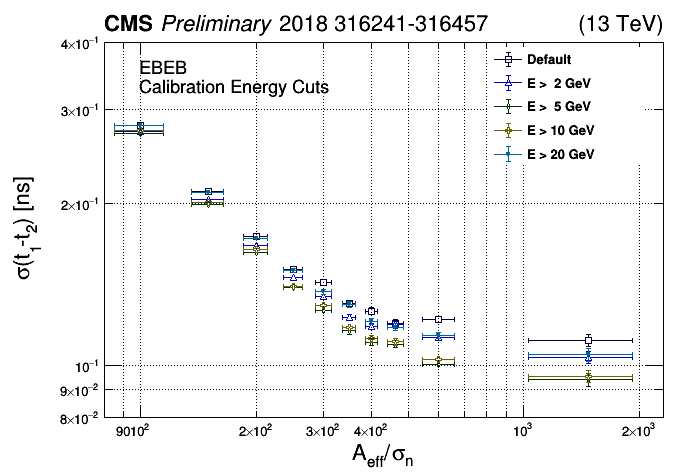
\includegraphics{fig/sec_method/tr_kucc_18s_ecut_v25_01122021174016.png}}
\caption{Same readout unit (SRU) resolution obtained with the default CMSSW timing reconstruction after applying an external calibration.
The calibration constants are derived by averaging rechit times on a channel-by-channel basis using rechits with energy greater than a specified threshold.}
\label{e5cali}
\end{center}
\end{figure}

To enable a consistent comparison between different ECAL timing reconstruction algorithms, rechit times must be calibrated using a common procedure.
During Run~II development, it was not possible to apply the default CMSSW timing calibration framework directly to rechits reconstructed with the CC algorithm.
An external calibration procedure based on the average rechit time per channel was therefore implemented.

In this approach, calibration constants are derived by computing the mean rechit time for each crystal over a selected set of events.
To suppress contributions from electronic noise and poorly reconstructed pulses, rechits used in the calibration are required to exceed a minimum energy threshold.
The dependence of the resulting timing resolution on this threshold was studied using the default CMSSW timing reconstruction in selected runs from the 2018D data-taking period.

As shown in Fig.~\ref{e5cali}, increasing the minimum rechit energy threshold above 5\,GeV yields negligible improvement in the calibrated time resolution.
Based on these studies, a threshold of 5\,GeV is chosen for the external calibration procedure.
This calibration is applied to all rechit times reconstructed with the CC algorithm throughout this analysis and is used consistently for Run~II studies prior to the introduction of a CC-specific calibration within CMSSW during Run~III.

For direct comparisons between the CC and ratio-based timing reconstructions, an analogous external calibration derived from rechit times reconstructed with the ratio method is also applied.
This ensures that both timing algorithms are calibrated using equivalent procedures and that observed differences in performance reflect intrinsic reconstruction behavior rather than calibration effects.
